\documentclass{report}

\usepackage{graphicx}
\title{Box Problem}
\author{Dries Rooryck}

\begin{document}
	
Written report on general proof behind the lower bound strategy for a uniform distribution.\\
 $n$ is the amount of boxes, and thus also the range of values that can be conatined inside these boxes (eg. 100 boxes have money between 1-100 dollars, 10 boxes have money between 1-10) \\
 $b$ is the value for the lower bound chosen,(eg. a lower bound of 8 means you only choose higher than 8) \\
 We can calculate the probability of winning using this equation.\\



\[ 
\textrm{P(win)} = \sum_{i=1}^{n} P ( \textrm{win in box } i) 
\]

\[
 \textrm{P (win in box  }i) = \sum_{j=0}^{(n-b)-1} P ( \textrm{ win in box } i \textrm{ with } n-j \textrm{ dollars}) 
 \]

\[
P ( \textrm{ win in box } i \textrm{ with } n-j \textrm{ dollars}) =
\left( \frac{1}{n} \right)\cdot \left( \frac{b}{n} \right)^{i-1}\cdot \left(\frac{n-j}{n} \right)^{n-i} 
\]


 \[
 \textrm{P(win)} =
 \sum_{i=1}^{n} \quad \left[ \sum_{j=0}^{(n-b)-1} \left( \frac{1}{n} \right)\cdot \left( \frac{b}{n} \right)^{i-1}\cdot \left(\frac{n-j}{n} \right)^{n-i} \right] 
 \]
	

On the following plots, the y axis is the theoretical probability of winning, whereas the x axis accounts for the value of the lower boundary chosen (b)
Here is a plot where $n=10$. 	\\
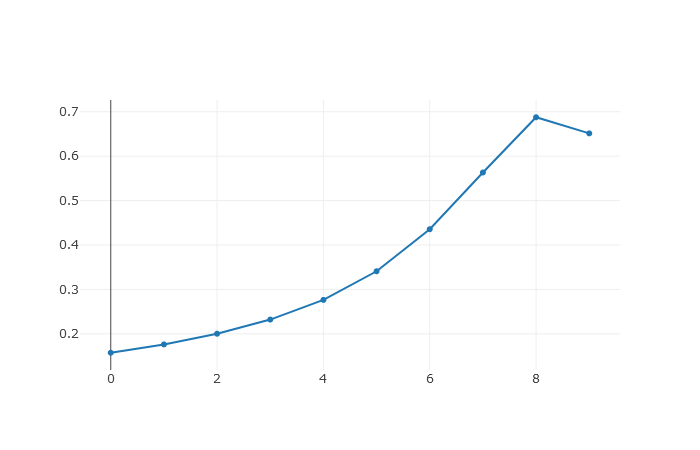
\includegraphics[scale=0.4]{newplot.png}

\pagebreak

Here is a plot where $n=100$ \\
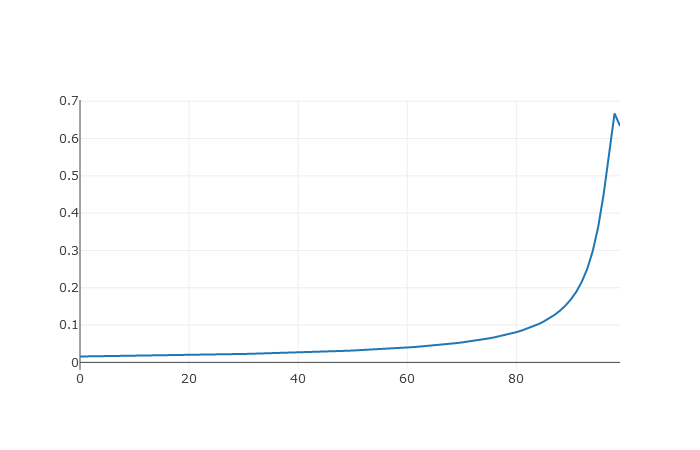
\includegraphics[scale=0.4]{100plot.png}

Here is the same plot, but the x axis (the lower boundary), only has values from 90 to 100 \\
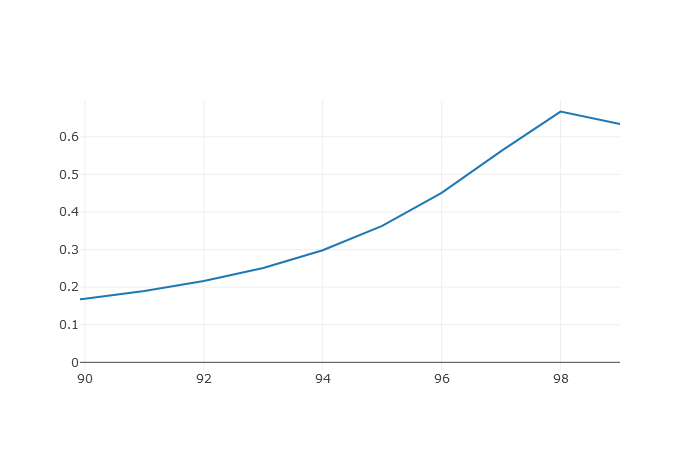
\includegraphics[scale=0.4]{90 100 plot.png}

\pagebreak

Here is a plot where $n=1000$ \\
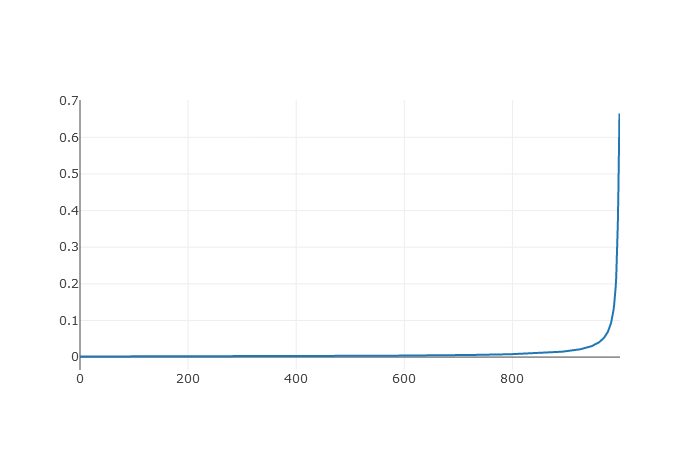
\includegraphics[scale=0.4]{1000 plot.png}

Here is the same plot, but the x axis (the lower boundary), only has values from 980 to 1000 \\
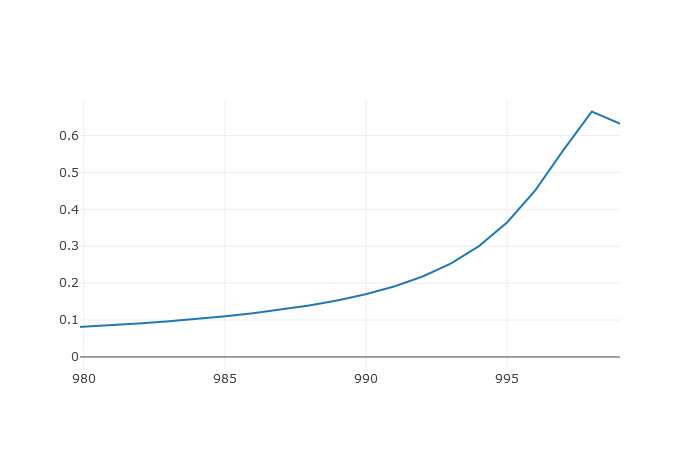
\includegraphics[scale=0.4]{980 1000 plot.png}

Observations: \\
The highest chance is always between 0.65 and 0.70 \\
The highest probabilty is always $n-2$, with n-1 being slightly lower. \\
The function describes a gentle slope




\end{document}